\documentclass[oneside,a4paper]{book}

\usepackage[pdftex]{graphicx}
\usepackage{amsmath}
\usepackage{amssymb}
\usepackage{textcomp}
\usepackage[utf8]{inputenc}
\usepackage[polish]{babel}
\usepackage[T1]{fontenc}
\usepackage{array}
\usepackage{tabularx}
\usepackage{enumitem}
\usepackage[justification=centering]{caption}

\raggedbottom

% pakiet stosowany do url'i w bibliografii, zamienia odnośniki na ładnie sformatowane
\usepackage{url}
% pakiety służące do numerowania i tworzenia algorytmów
\usepackage{algorithmic}
\usepackage{algorithm}
% redefinicja etykiety nagłówkowej listy algorytmów, domyślna jest po angielsku
\renewcommand{\listalgorithmname}{Spis algorytmów}

% pakiet do wyliczania skali, przydatny przy dużych obrazkach
\usepackage{pgf}
% pakiet służący do automatycznego sortowania odnośników do bibliografii
\usepackage[sort]{natbib}
% tworzenie listingów
\usepackage{listings}
% tworzenie figur wewnątrz figur
\usepackage{subfig}
% do automatycznego skracania nazw rozdziałów i podrozdziałów używanych w nagłówkach strony by mieściły się w jednej linii
\usepackage[fit]{truncate}
% fancyhdr - ładne nagłówki, definicja wyglądu nagłówka, numery stron będą umieszczane w nagłówku po odpowiedniej stronie
\usepackage{fancyhdr}
\pagestyle{fancy}
\renewcommand{\chaptermark}[1]{\markboth{#1}{}}
\renewcommand{\sectionmark}[1]{\markright{\thesection\ #1}}
\fancyhf{}
\fancyhead[LE,RO]{\bfseries\thepage}
% tutaj ograniczamy szerokość pola w nagłówku zawierającego nazwę rozdziału/podrozdziału do 95% szerokości strony
% redefinicja sposobu prezentacji nazw domyślnie wypisywanych wielkimi literami (np. domyślnie w nagłówku Spis treści będzie miał postać SPIS TREŚCI)
% Uwaga! to może popsuć wielkie litery w ogóle! Jak coś nie działa należy usunąć \nouppercase{} z poniższych definicji
\fancyhead[LO]{\nouppercase{\bfseries{\truncate{.95\headwidth}{\rightmark}}}}
\fancyhead[RE]{\nouppercase{\bfseries{\truncate{.95\headwidth}{\leftmark}}}}
\renewcommand{\headrulewidth}{0.5pt}
\renewcommand{\footrulewidth}{0pt}

% definicja typu prostego wymagana przez pierwsze strony rozdziałów itp.
% powyższe reguły niestety tych stron nie dotyczą, gdyż Latex automatycznie przełącza je pomiędzy fancy a plain
% w tym wypadku eliminujemy nagłówki i stopki na stronach początkowych
\fancypagestyle{plain}{%
 \fancyhead{}
 \fancyfoot{}
 \renewcommand{\headrulewidth}{0pt}
 \renewcommand{\footrulewidth}{0pt}
}

%\parskip 0.5in

% makro umożliwiające otaczanie symboli okręgami
\usepackage{tikz}
% brak justowania tekstu (bazą okręgu będzie linia tekstu)
\newcommand*\mycirc[1]{%
  \begin{tikzpicture}
    \node[draw,circle,inner sep=1pt] {#1};
  \end{tikzpicture}}

% pionowe justowanie tekstu, środek okręgu pokrywa się ze środkiem tekstu
\newcommand*\mycircalign[1]{%
  \begin{tikzpicture}[baseline=(C.base)]
    \node[draw,circle,inner sep=1pt](C) {#1};
  \end{tikzpicture}}

% zmiana nazwy twierdzeń i lematów
\newtheorem{theorem}{Twierdzenie}[section]
\newtheorem{lemma}[theorem]{Lemat}

% tworzenie definicji dowodu
\newenvironment{proof}[1][Dowód]{\begin{trivlist}
\item[\hskip \labelsep {\bfseries #1}]}{\end{trivlist}}
% \newenvironment{definition}[1][Definicja]{\begin{trivlist}
% \item[\hskip \labelsep {\bfseries #1}]}{\end{trivlist}}
% \newenvironment{example}[1][Przykład]{\begin{trivlist}
% \item[\hskip \labelsep {\bfseries #1}]}{\end{trivlist}}
% \newenvironment{remark}[1][Uwaga]{\begin{trivlist}
% \item[\hskip \labelsep {\bfseries #1}]}{\end{trivlist}}

% definicja czarnego prostokąta zwyczajowo dodawanego na koniec dowodu
\newcommand{\qed}{\nobreak \ifvmode \relax \else
      \ifdim\lastskip<1.5em \hskip-\lastskip
      \hskip1.5em plus0em minus0.5em \fi \nobreak
      \vrule height0.75em width0.5em depth0.25em\fi}

% poniższymi instrukcjami można sterować co ma być numerowane a co nie i co ma być wyświetlane w spisie treści
% \setcounter{secnumdepth}{3}
% \setcounter{tocdepth}{5}

% definicja czcionki mniejszej niż tiny (domyślnie takiej małej nie ma)
\usepackage{lmodern}
\makeatletter
  \newcommand\tinyv{\@setfontsize\tinyv{4pt}{6}}
\makeatother

% definicja jeszcze mniejszej czcionki
\usepackage{lmodern}
\makeatletter
  \newcommand\tinyvv{\@setfontsize\tinyvv{3.5pt}{6}}
\makeatother

% pakiet do obsługi wielostronicowych tabel
\usepackage{longtable}
\setlength{\LTcapwidth}{\textwidth}

\usepackage[section] {placeins}
\usepackage{multirow}
\usepackage{slantsc}

% interlinia
\usepackage{setspace}

% korekta marginesów - domyślnie latex ma jakieś kosmiczne
\usepackage{anysize}
\marginsize{3.5cm}{2.5cm}{2.5cm}{2.5cm}
% po zmianie marginesów konieczne jest wymuszenie przeliczenia nagłówków
\fancyhfoffset[E,O]{0pt}

\usepackage{titlesec}
\titlespacing*{\chapter}{0pt}{-50pt}{20pt}
\titleformat{\chapter}[display]{\normalfont\huge\bfseries}{\chaptertitlename\ \thechapter}{20pt}{\huge}

\setlength{\LTleft}{0pt}
\setlist[itemize]{nolistsep}
\setlist[enumerate]{nolistsep}
\begin{document}

\begin{titlepage}
\begin{center}

% Nagłówek

\includegraphics[width=0.3\textwidth]{img/put_logo.png}\\[0.1in]
\Large{Instytut Informatyki}\\
\normalsize
Wydział Informatyki\\
Politechnika Poznańska\\
ul. Piotrowo 2, Poznań \\[2cm]

\Large{PRACA DYPLOMOWA MAGISTERSKA}\\[1cm]

% Title
\Large \textbf {System wspomagający jednoczesne stosowanie wielu procedur klinicznych dla jednego pacjenta}\\[2cm]
% Submitted by
\begin{table}[h]
\centering
\begin{tabular}{lr}\hline \\ 
Dariusz Radka & 100383 \\ \\ \hline 
\end{tabular}
\end{table}

\vspace{1cm}

\normalsize Promotor \\
\begin{table}[h]
\centering
\begin{tabular}{c}\hline \\
dr hab. inż. Szymon Wilk \\ \\ \hline 
\end{tabular}
\end{table}

\vspace{2cm}
Poznań, 2015

\vfill

\end{center}

\end{titlepage}

% sekcja wstępna książki, numerowana rzymskimi
\frontmatter
% generacja strony tytułowej załączonej wcześniej
% \maketitle
% spis treści
\tableofcontents

% dodatkowa strona z podaniem źródła finansowania itp.
% wstawienie pustego symbolu
\null
% i wypełnienie nim całej dostępnej strony
\vfill
% a na jej dole dodajemy właściwy tekst
% w tym przypadku z wyrównaniem do prawej strony

% właściwa część książki, numerowana arabskimi od 1
\mainmatter
\def\arraystretch{1.5}

\chapter{Wstęp}
\section{Wprowadzenie}

\begin{spacing}{1.5}
Medycyna jest ważnym działem nauki, ponieważ dotyczy każdego człowieka. Pozwala na wyleczenie ludzi z różnych chorób przy zastosowaniu odpowiedniej terapii, doborze odpowiednich lekarstw itp. Istotne znaczenie przy leczeniu pacjenta ma wiedza, jaką dysponuje lekarz. Informatyka, która jest dziedziną nauki zajmującą się przetwarzaniem informacji, może pomóc lekarzom w zdobywaniu wiedzy. Dzięki systemom korzystającym z baz danych zawierających opisy leków, chorób, procedur medycznych oraz danych dotyczących pacjentów można w łatwiejszy sposób dobrać odpowiednią terapię dla pacjenta, co ma istotny wpływ na przebieg jego leczenia. Przykładem takiego systemu medycznego jest Eskulap. Jest to system zrealizowany przez pracowników Politechniki Poznańskiej. Eskulap jest skierowany dla różnych placówek medycznych, m. in. szpitali, przychodni oraz aptek. Korzysta z niego wiele placówek na terenie całej Polski. Eskulap składa się z kilkudziesięciu modułów. Do modułów tych należą m. in. eRejestracja, Apteka, Laboratorium, Elektroniczna Dokumentacja Medyczna. Innym przykładem systemu medycznego jest InfoMedica. Jego głównym zadaniem jest ewidencja świadczeń zdrowotnych. System przechowuje informacje o chorych, używanych lekach oraz materiałach wykorzystywanych w placówkach medycznych. Dzięki systemowi InfoMedica możliwa jest również ewidencja finansowo-księgowa oraz kadrowo-płacowa. 
Pacjenci często chorują na nie tylko jedną przypadłość, ale muszą leczyć się z kilku dolegliwości. W przypadku takich pacjentów konieczne jest dobranie leków, które nie pozostają ze sobą w konflikcie. Jeśli takie konflikty występują, należy znaleźć odpowiedni zamiennik lub przepisać dodatkowy lek. W niektórych przypadkach trzeba zrezygnować z leków, aby nie pogorszyć stanu zdrowia pacjenta. Zadaniem systemu, którego dotyczy niniejsza praca magisterska, jest znajdowanie konfliktów wynikających ze stosowania wielu terapii u jednego pacjenta. W przypadku znalezienia konfliktu, należy dokonać zmian w procedurze medycznej tak, aby zminimalizować skutki uboczne. 


\section{Cel i zakres pracy}

Celem pracy magisterskiej jest realizacja systemu pozwalającego na kontrolowane stosowanie kilku procedur medycznych dla jednego pacjenta. System ten ma wykorzystywać programowanie logiczne z ograniczeniami. Wybranym językiem programowania dla wykonania tego systemu jest język Java. System ma pozwalać na korzystanie z procedur medycznych w sposób krokowy polegający na udzielaniu odpowiedzi na pytania. Na początku system wyświetla listę chorób. Należy z nich wybrać te choroby, na które choruje pacjent. Po wybraniu chorób system pozwala na udzielanie odpowiedzi na pytania wchodzące w skład procedur medycznych związanych z wybranymi chorobami. Podczas udzielania odpowiedzi na grafie opisującym określoną procedurę medyczną zaznaczana jest ścieżka, którą wybieramy. W następnej fazie system znajduje ewentualne konflikty wynikające ze stosowania kilku procedur medycznych. Konflikty te mogą dotyczyć użytych leków, stosowanych terapii lub dolegliwości, na które choruje pacjent . Wyszukiwanie konfliktów jest oparte na programowaniu logicznym z ograniczeniami. Wykorzystywana jest do tego celu biblioteka o nazwie Choco w wersji 3. Jest to biblioteka napisana dla języka Java. System po znalezieniu konfliktu wprowadza poprawki do procedur medycznych. Poprawki te mogą polegać na dodaniu lub usunięciu jakiegoś elementu z procedury, a także mogą polegać na zamianie jednego elementu na inny. Poprawione procedury medyczne są prezentowane w postaci  grafów. Grafy te podobne są do grafów prezentujących ścieżki, które wybraliśmy podczas udzielania odpowiedzi na pytania z tą różnicą, że grafy wynikowe posiadają wprowadzone zmiany w elementach, jeśli zostały znalezione konflikty. Ponadto, grafy wynikowe zawsze posiadają ścieżkę, dla której ostatnim elementem jest zdarzenie końcowe. Procedury medyczne są zapisane w formacie Graphviz o rozszerzeniu dot. Za pomocą programu dot.exe z plików o rozszerzeniu dot generowane są obrazy przedstawiające grafy procedur medycznych. 

\section{Struktura pracy}

W rozdziale 2 zamieszczono przegląd literatury na temat wytycznych postępowania klinicznego oraz ich roli w medycynie. W tym rozdziale zaprezentowano także podejścia do wykrywania i usuwania interakcji w wytycznych postępowania klinicznego. Rozdział 3 opisuje paradygmat programowania logicznego z ograniczeniami. Opisano w tym rozdziale podstawowe właściwości tego sposobu programowania, a także zamieszczono przykład ilustrujący wykorzystanie programowania logicznego z ograniczeniami w praktyce. W rozdziale 4 zaprezentowano narzędzia i biblioteki użyte podczas wykonywania pracy magisterskiej. Rozdział 5 opisuje główną część pracy, czyli implementacje systemu. W tym rozdziale przedstawiono poszczególne części systemu. Rozdział 6 prezentuje przykładowe działanie systemu. Rozdział 7 stanowi podsumowanie pracy. 

\chapter{Przegląd literatury}
\section{Wytyczne postępowania klinicznego}

Wytyczne postępowania klinicznego\cite{Boyd, Latoszek-Berendsen} pozwalają polepszyć jakość opieki medycznej. Wytyczne są tworzone przez ekspertów medycznych. Rozwój wytycznych wysokiej jakości wymaga specjalistycznego zespołu ludzi i wystarczającego budżetu. Wytyczne powinny oferować spersonalizowane porady. Komputerowo interpretowane wytyczne, które posiadają dostęp do elektronicznego rekordu pacjenta, są w stanie dostarczyć porady dotyczące konkretnego pacjenta. Wytyczne wpływają pozytywnie na pracę personelu medycznego i zwiększają wydajność. Pacjenci mogą czerpać korzyści z wytycznych, które podsumowują zalety i wady możliwych opcji. Pacjenci mogą się dowiedzieć więcej o wyborach medycznych, które uwzględniają ich osobistą charakterystykę. Cały system medyczny może dzięki wytycznym zwiększyć wydajność, co może obniżyć koszty usług, przepisywanych leków czy zlecanych badań. Wytyczne w przypadku pacjentów chorujących na kilka chorób, którymi często są osoby starsze, mogą doprowadzić do niewłaściwego wyboru terapii. Ważnym aspektem w tej kwestii jest znajdowanie konfliktów występujących między wytycznymi i ich odpowiedniego rozwiązania.

\section{Wykrywanie i usuwanie interakcji w wytycznych postępowania klinicznego}

\subsection{Logika pierwszego rzędu}

Wytyczne postępowania klinicznego są w tej technice prezentowane w postaci grafu akcji.\cite{SzWilk} Graf akcji jest grafem skierowanym, na który składają się trzy typy węzłów. Pierwszy typ to węzeł kontekstu. Jest to węzeł początkowy opisujący określoną chorobę. Kolejnym typem jest węzeł akcji, który opisuje akcję medyczną, którą należy wykonać. Ostatnim typem jest węzeł decyzji, który zawiera pytanie, na które należy odpowiedzieć. Słownictwo podejścia logiki pierwszego rzędu składa się ze stałych (pisanych dużymi literami), zmiennych (pisanych małymi literami) oraz predykatów. Do predykatów należą:
\begin{itemize}
\item{node(x) – x jest węzłem}
\item{action(x) – x jest węzłem akcji}
\item{decision(x) – x jest węzłem decyzji}
\item{executed(x) – węzeł akcji x jest zastosowany}
\item{value(x, v) – wartość v jest związana z węzłem decyzji x}
\item{dosage(x, n) – węzeł akcji x jest opisany przez dawkę n}
\item{directPrec(x, y) – węzeł x poprzedza bezpośrednio węzeł y}
\item{prec(x, y) – węzeł x poprzedza węzeł y}
\item{disease(d) – d jest chrobą}
\item{diagnosed(d) – pacjent choruje na chorobę d}
\end{itemize}
W tym podejściu stosowane są także tzw. operatory interakcji i rewizji. Operator interakcji reprezentuje niepożądany konflikt (zazwyczaj lek-lek lub lek-choroba), który jest w postaci zdania zbudowanego za pomocą powyższych predykatów. Operator rewizji natomiast składa się z dwóch części. Pierwsza część jest podobna do operatora interakcji, również zbudowana jest ze zdania opisującego konflikt, który może wystąpić. Druga część składa się z par formuł, które opisują pojedyncze interakcje operatora. Pary formuł mogą być w trzech postaciach:
\begin{itemize}
\item{(x, $\emptyset$) – oznacza, że formuła x jest usuwana}
\item{($\emptyset$, x) – oznacza, że formuła x jest dodawana}
\item{(x, y) – oznacza, że formuła x jest zamieniana na formułę y}
\end{itemize}


\subsection{Podejście Piovesana}

Wytyczne w tym podejściu są reprezentowane w postaci hierarchicznego grafu składającego się z węzłów będących akcjami i krawędzi modelujących relacje między akcjami.\cite{Piovesan} Podejście rozróżnia akcje atomowe i akcje złożone (plany). Na akcje atomowe składa się pięć typów:
\begin{itemize}
\item{Akcje pracy – opisują zewnętrzne akcje}
\item{Akcje farmaceutyczne – opisują przepisane leki i ich dawki}
\item{Akcje decyzji – reprezentują wybór spośród różnych alternatyw}
\item{Akcje zapytań – są związane z żądaniami informacji (zazwyczaj danych pacjenta)}
\item{Konkluzje – modelują wyniki akcji decyzji}
\end{itemize}
Ontologie wykorzystywane w tym podejściu są mocno zintegrowane z obecnymi ontologiami medycznymi, takimi jak SNOMED CT dla pojęć medycznych i ATC dla klasyfikacji leków. Akcje złożone, pracy i farmaceutyczne są reprezentowane na dwóch poziomach: za pomocą prototypu akcji (o nazwie Action), który jest charakteryzowany przez efekty (krawędź hasEffect) i przepisane leki (krawędź substance), i akcji specyficznej dla CIG (komputerowo interpretowanych wytycznych) o nazwie CIGaction, która dziedziczy wszystkie własności z prototypu, ale dodatkowo zawiera intencję akcji (krawędź aimsTo). Ponadto wyróżniamy modyfikację (o nazwie Variation) modelowaną za pomocą zmian (krawędź hasModality, pojęcie Modality) atrybutu (krawędź focusOn, pojęcie Attribute). Zmiany należą do zbioru: „Increase” (zwiększ), „Decrease” (zmniejsz), „Stability” (bez zmian). Ponadto, możliwe jest określenie interakcji między dwiema lub więcej modyfikacjami (pojęcie VariationInteraction). Interakcja jest scharakteryzowana przez typ (krawędź hasType), którego wartości należą do zbioru: „Concordance” (zgodność), „Discordance” (niezgodność), „Independence” (niezależność). Interakcja między intencjami (pojęcie IntentionInteraction) jest specyficznym rodzajem interakcji między modyfikacjami (pojęcie VariationInteraction), która uwzględnia przynajmniej jedną intencję. Interakcje pomiędzy lekami (pojęcie DrugInteraction) są związane ze zmianami (krawędź hasModality), które powoduje interakcja w modyfikacji określonej krawędzią „changes”. Często interakcja między dwoma lekami jest spowodowana interakcją pomiędzy dwoma ich efektami. Do zamodelowania takiej informacji wykorzystana zostaje własność „causedBy” odnosząca się do pojęcia „VariationInteraction”. Ponadto, dla akcji, modyfikacji i intencji można dołączyć informację o czasie (krawędź happens, pojęcie TemporalEntity).

W podejściu Piovesana wykorzystywane są także opcje, które pozwalają zarządzać interakcjami. Do opcji tych należą m. in. bezpieczna alternatywa oraz tymczasowe unikanie. Bezpieczna alternatywa polega na wyborze alternatywnej ścieżki w wytycznych, która unika interakcji. Tymczasowe unikanie polega natomiast na stosowaniu leków w takich momentach czasu, w których nie występuje interakcja pomiędzy nimi.

\chapter{Programowanie logiczne z ograniczeniami (CLP)}

Programowanie logiczne z ograniczeniami\cite{CLP} jest rodzajem programowania z ograniczeniami, w którym programowanie logiczne jest rozszerzone o koncepcję spełnienia ograniczeń. Przykładowym ograniczeniem może być wyrażenie postaci X+Y>5. 
Ogólnie przypadek CLP składa się z następujących cech:
\begin{itemize}
\item{Skończonego zbioru zmiennych typu całkowitoliczbowego z wartościami ze skończonych dziedzin}
\item{Zbioru ograniczeń między zmiennymi}
\item{Rozwiązań problemu polegających na przypisaniu wartości do zmiennych, które spełniają ograniczenia}
\end{itemize}
Przykładowym zastosowaniem programowania logicznego z ograniczeniami jest zagadka SEND + MORE  = MONEY.\cite{Eclipse} Zagadka ta polega na przypisaniu cyfr z zakresu od 0 do 9 do zmiennych odpowiadających literom zawartym w równaniu tak, aby równanie było spełnione. Każda litera ma swoją unikalną wartość cyfrową. Ponadto litery S i M mają wartości różne od 0.
\begin{verbatim}
    SEND
  + MORE
 -------
   MONEY
\end{verbatim}
\newpage
Rozwiązaniem tego problemu jest następujący program napisany w ECLiPSe:
\begin{verbatim}
:-lib(ic).
sendmore1(Digits):-
Digits = [S,E,N,D,M,O,R,Y],
Digits :: [0..9],
alldifferent(Digits),
S #\= 0,
M #\= 0,
1000*S + 100*E + 10*N + D
+ 1000*M + 100*O + 10*R + E
#= 10000*M + 1000*O + 100*N + 10*E + Y,
labeling(Digits).
\end{verbatim}
Po skompilowaniu tego programu w narzędziu TkEclipse wystarczy wywołać funkcję sendmore1(Digits), aby otrzymać rozwiązanie zagadki.


\chapter{Wykorzystane biblioteki i narzędzia}

\section{ECLiPSe}

ECLiPSe\cite{EclipseSite} jest systemem typu open-source do tworzenia aplikacji wykorzystujących paradygmat programowania logicznego z ograniczeniami. System ten użyty został do testowania przykładowych procedur medycznych. Nie współpracuje natomiast z wykonanym w ramach pracy magisterskiej systemem, jest to odrębny program. ECLiPSe składa się z trzech części. Pierwsza część służy do wprowadzania komend. Zamiast wprowadzania komend można wczytać gotowy program z pliku za pomocą polecenia Compile znajdującym się w menu File. Druga część programu wyświetla wyniki, trzecia natomiast pokazuje ewentualne błędy oraz inne komunikaty. Komendy dla tego systemu składają się ze zdań zakończonych kropką, poszczególne fragmenty zdań są oddzielone od siebie przecinkami. Znak równości to między zmiennymi lub wartościami liczbowymi to „\#=”, znak nierówności to „\#\textbackslash=”. Można stosować także operatory and i or i przypisywać ich wartość do zmiennych za pomocą znaku równości. 

\section{Choco 3}

Choco\cite{Choco3} jest darmowym oprogramowaniem typu open-source wykorzystującym paradygmat programowania z ograniczeniami. Jest to biblioteka oparta o język Java w wersji 8. Główną klasą biblioteki jest klasa Solver. Do obiektu typu Solver można dołączyć zmienną (klasa IntVar) podając obiekt Solvera w ostatnim argumencie metody bounded klasy VariableFactory. Pozostałe argumenty tej metody to nazwa zmiennej oraz dolne i górne ograniczenie zmiennej. W pracy magisterskiej wykorzystywane są w większości zmienne, dla których dolne ograniczenie jest równe 0, a górne ograniczenie jest równe 1, czyli są to zmienne przyjmujące wartości prawda/fałsz. Za pomocą funkcji post solvera można dodawać nowe ograniczenia. Ograniczenia tworzy się m. in. za pomocą klasy IntConstraintFactory. Jedną z podstawowych funkcji tworzących ograniczenia jest funkcja arithm. Przykładowo, można za jej pomocą określić, że suma dwóch zmiennych X i Y ma być mniejsza od 5. Po określeniu ograniczeń można uruchomić solver i wygenerować rozwiązanie za pomocą funkcji solvera o nazwie findSolution. Kolejne rozwiązania można uzyskać za pomocą funkcji nextSolution. Odczytanie wartości zmiennej określonego rozwiązania polega na wywołaniu funkcji zmiennej o nazwie getValue. 

\section{JPGD - A Java parser for Graphviz documents}

Biblioteka\cite{JPGD} ta służy do konwersji pliku o rozszerzeniu dot opisującego graf procedury medycznej na obiekt klasy Graph posiadający listę obiektów klasy Node oraz Edge. Do konwersji wykorzystywany jest obiekt klasy Parser. Klasa Parser posiada funkcję parse, której konstruktor jako parametr przyjmuje obiekt klasy FileReader odwołujący się do określonego pliku o rozszerzeniu dot. W następnym kroku można odczytać obiekt klasy Graph z listy tych obiektów uzyskanej za pomocą funkcji getGraphs (jest to funkcja klasy Parser). Węzły grafu można odczytać za pomocą funkcji getNodes wywołanej dla obiektu klasy Graph. Krawędzie grafu można natomiast uzyskać za pomocą funkcji getEdges, która również jest funkcją klasy Graph. Węzły oraz krawędzie posiadają atrybuty. Do atrybutów węzłów należy zaliczyć etykietę, kształt, kolor wypełnienia, kolor konturu i grubość linii konturu. Krawędzie posiadają przede wszystkim jeden istotny atrybut – etykietę. Odczytać wartości atrybutów można za pomocą funkcji getAttribute, której argumentem jest nazwa atrybutu. Ustawić wartości atrybutu można natomiast za pomocą metody setAttribute, której pierwszym argumentem jest nazwa atryubutu, a drugim jego wartość. Każdy węzeł grafu będącym w formacie dot posiada także swój unikalny identyfikator. Identyfikatory przechowywane są w obiektach klasy Id. Obiekt takiej klasy dla określonego węzła można uzyskać wywołując funkcję getId() na rzecz obiektu klasy Node. Ponowne wywołanie funkcji getId, w tym przypadku dla obiektu klasy Id uzyskuje rzeczywisty identyfikator węzła typu String. Jeśli chodzi o krawędzie, to posiadają one możliwość odczytania węzła źródłowego oraz docelowego danej krawędzi. Jest to możliwe dzięki wywołaniu funkcji getSource (dla uzyskania węzła źródłowego) oraz getTarget (dla uzyskania węzła docelowego). Dzięki tym funkcjom uzyskujemy obiekt klasy PortNode, z którego następnie możemy uzyskać obiekt klasy Node za pomocą funkcji getNode. Ważną funkcją jest też funkcja toString wywoływana na rzecz obiektu klasy Graph. Pozwala ona na uzyskanie grafu w formacie dot zawierającym zmiany wprowadzone za pomocą metody setAttribute dla obiektów klasy Node lub Edge. Aby wygenerowany graf był poprawny, konieczna była modyfikacja metody toString dla klas Graph, Node oraz Edge, gdyż biblioteka zawiera w przypadku tych metod drobne błędy. Po uzyskaniu grafu w formacie dot można go następnie zapisać do pliku, aby móc z niego później skorzystać.

\section{Graphviz}

Graphviz\cite{Graphviz} jest oprogramowaniem służącym do wizualizacji grafów. Pozwala na konwersję pliku tekstowego o rozszerzeniu dot do obrazu przedstawiającego graf. Program automatycznie porządkuje węzły na obrazie, nie jest konieczne podawanie pozycji węzłów, czyli ich współrzędnych x i y. Program Graphviza o nazwie gvedit.exe jest programem okienkowym, który pozwala na wybranie w oknie dialogowym pliku o rozszerzeniu dot. Po wybraniu tego pliku albo wypisywana jest lista błędów, które należy poprawić, albo wyświetlany jest obraz przedstawiający graf. Podobną funkcjonalność ma program dot.exe, z tą różnicą, że jest to program konsolowy. Program dot.exe posiada 3 argumenty. Pierwszym argumentem jest ścieżka do pliku z rozszerzeniem dot, drugim jest format generowanego obrazu (przykładowo dla uzyskania formatu png obrazka podajemy drugą wartość argumentu równą –Tpng). Między drugim a trzecim argumentem należy podać przełącznik „-o”. Trzecim argumentem jest ścieżka wynikowego obrazu. Jeśli chodzi o plik z rozszerzeniem dot, jest to plik, który posiada swoją własną składnię. Na początku pliku umieszczone jest słowo „digraph”, po którym umieszcza się nazwę grafu. Wszystkie pozostałe właściwości grafu są umieszczone w bloku otoczonym nawiasami klamrowymi. W bloku tym można podać globalne atrybuty dla węzłów oraz krawędzi. Atrybuty dla węzłów mogą być podane po słowie node w bloku otoczonym nawiasami kwadratowymi, atrybuty są oddzielone od siebie przecinkami. Do przykładowych globalnych atrybutów węzłów należą m. in. kształt (box – prostokąt, circle – koło, diamond – romb), kolor wypełnienia, kolor konturu, grubość linii konturu, rodzaj czcionki, wielkość czcionki. Jeśli chodzi o globalne atrybuty krawędzi, to można je podać w podobny sposób jak globalne atrybuty węzłów, z tą różnicą, że zamiast słowa „node” należy podać słowo „edge”. Do atrybutów globalnych krawędzi należą przede wszystkim wielkość i rodzaj czcionki (krawędzie mogą posiadać etykiety). W następnym kroku można podać węzły i krawędzie z ich atrybutami. Atrybut pojedynczego węzła lub krawędzi, jeśli już wystąpił w globalnych atrybutach węzłów lub krawędzi, zostaje nadpisany. Opis pojedynczego węzła polega na podaniu jego unikalnego identyfikatora, a następnie jego atrybutów w bloku otoczonym nawiasami kwadratowymi (atrybuty są podawane po przecinku).  Krawędzie natomiast tworzy się, podając na początku identyfikator węzła źródłowego krawędzi, następnie należy umieścić tzw. strzałkę („->”), a na końcu identyfikator węzła docelowego. Po podaniu tych elementów można podać atrybuty krawędzi, przede wszystkim etykietę. Co ciekawe, krawędź może być także nieskierowana, wtedy zamiast strzałki („->”) należy umieścić podwójną kreskę („--”). 
W systemie, którego dotyczy praca magisterska, wykorzystano program dot.exe. Za pomocą funkcji getRuntime klasy Runtime uzyskujemy instancję obiektu klasy Runtime. Na rzecz tego obiektu można następnie wywołać funkcję exec, której argumentem jest tablica łańcuchów znaków zawierająca w pierwszym elemencie ścieżkę do programu (w tym przypadku dot.exe), a w pozostałych elementach argumenty programu. Następnie należy wywołać funkcję waitFor dla obiektu klasy Process, który uzyskujemy w wyniku wywołania funkcji exec.

\chapter{Implementacja}

\section{Struktura katalogów}

\begin{itemize}
\item{Algorytmy – zawiera pliki o rozszerzeniu dot opisujące grafy procedur medycznych chorób}
\item{Konflikty – zawiera opisy konfliktów, jakie występują między chorobami oraz zmiany, które należy wprowadzić w przypadku wystąpienia konfliktów}
\item{Grafy – zawiera zmodyfikowane grafy chorób przedstawiające aktualnie przebytą ścieżkę oraz grafy wynikowe prezentujące rozwiązania. Grafy są w dwóch formatach – tekstowym w formacie dot oraz graficznym w formacie png. Po zamknięciu programu zawartość tego katalogu jest kasowana}
\end{itemize}

\section{Wybór chorób}

W katalogu algorytmy program szuka plików posiadających rozszerzenie dot. Dla każdego takiego pliku tworzony jest checkbox. Checkbox posiada etykietę równą nazwie choroby. Utworzony checkbox jest następnie dodawany do globalnej listy checkboxów o nazwie checkBoxGroup oraz do panela znajdującego się w lewym górnym rogu programu. Po wybraniu chorób, tzn. po kliknięciu w odpowiednie checkboxy i kliknięciu przycisku „Dalej”, nazwy wybranych chorób są dodawane do listy o nazwie selectedDiseases i program przechodzi do fazy wyświetlania grafów. 

\section{Wyświetlanie grafów}

Na początku program odczytuje z funkcji getGraph graf znajdujący się w pliku o rozszerzeniu dot oraz pobiera węzeł początkowy grafu. Operacje te wykonywane są dla każdej z wybranych chorób. Funkcja getGraph korzysta z funkcji parse obiektu klasy Parser należącego do biblioteki JPGD. Po odczytaniu grafu za pomocą funkcji getStartNode program znajduje węzeł początkowy grafu. Znalezienie takiego węzła polega na wyszukaniu węzła, który nie posiada krawędzi wejściowej. Następnie dla każdej choroby wywoływane są funkcje execute, newImageGraph oraz createRadioButtonList. Pierwsza z nich przemieszcza się po grafie, aby odnaleźć pierwsze pytanie w procedurze medycznej, oraz wywołuje funkcję color, która zaznacza przebytą ścieżkę. Podczas poruszania się po grafie do listy list o nazwie dataIdList dodawane są identyfikatory węzłów, na które program natrafił. Dzięki dataIdList funkcja color może pokolorować kontury przebytych węzłów oraz przebyte krawędzie, a także je pogrubić. Funkcja ta dla każdego elementu terapii określonej choroby znajdującego się w dataIdList szuka w grafie węzła posiadającego identyfikator o tej samej wartości, co element terapii lub węzła, którego identyfikator jest równy części elementu terapii przed znakiem zapytania. Element terapii dla węzłów, przy których udziela się odpowiedzi na pytania, składa się z dwóch części. W pierwszej z nich znajduje się identyfikator węzła, natomiast w drugiej etykieta krawędzi, która została wybrana. Obie części są oddzielone od siebie znakiem zapytania. W przypadku, gdy element terapii nie posiada znaku zapytania, zaznaczany jest znaleziony węzeł oraz wszystkie jego krawędzie wyjściowe.  Jeśli element terapii posiada znak zapytania, zaznaczany jest znaleziony węzeł oraz krawędź, której etykieta jest równa części elementu terapii po znaku zapytania.
 
Po wywołaniu funkcji color wywołana zostaje funkcja newImageGraph, której zadaniem jest umieszczenie na etykiecie podanej jako parametr określonego obrazu grafu. Na początku funkcja zapisuje do pliku wynik funkcji toString wywołanej dla grafu (wynik funkcji toString należało poprawić, biblioteka JPGD zawiera drobne błędy). Następnie wywoływana jest funkcja getImageGraphPath, która uruchamia program dot.exe i tworzy z zapisanego wcześniej pliku tekstowego graf w postaci obrazu. W kolejnym kroku funkcja newImageGraph tworzy obiekt klasy BufferedImage z wygenerowanym w poprzednim kroku obrazem. Później funkcja dokonuje skalowania obrazu tak, aby mógł on się zmieścić na etykiecie (JLabel). Jeśli szerokość lub wysokość obrazu przekracza 900 pikseli, obraz zmniejszany jest do 2/3 wielkości tak, aby był on czytelny (w tym przypadku do etykiety dodawane są suwaki).
 
Ostatnim krokiem jest wywołanie funkcji createRadioButtonList. Funkcja ta dla każdego elementu terapii, który posiada znak zapytania tworzy panel. Pierwszym elementem panelu jest etykieta węzła. Pozostałe elementy stanowią radiobuttony z etykietami, których wartości są równe etykietom krawędzi węzła z pytaniem. Do tych radiobuttonów dodawany jest jeszcze jeden z etykietą „brak wartości”. Część elementu terapii po znaku zapytania pozwala na wybranie aktywnego radiobuttona. Na końcu tworzony jest jeszcze jeden panel, tym razem dla pytania, na które jeszcze nie została udzielona odpowiedź, dla niego zaznaczony jest radiobutton z etykietą „brak wartości”. Przy pierwszym wyświetleniu grafu tworzony jest tylko ten panel. Ponadto, dla każdego radiobuttona przypisywane jest zdarzenie updateRadioButtonList.
 
Ostatecznie grafy prezentowane są po prawej stronie ekranu na zakładkach. Każda zakładka dotyczy jednej wybranej na początku programu choroby. Z lewej strony ekranu pojawiają się natomiast zakładki z listami radiobuttonów. W tym przypadku również jedna zakładka dotyczy pojedynczej choroby. Listy radiobuttonów pozwalają na udzielanie odpowiedzi na pytania zawarte w procedurach medycznych.


\section{Udzielanie odpowiedzi na pytaniaa}

Po kliknięciu na jeden z radiobuttonów uruchamiana jest procedura updateRadioButtonList. Na początku procedura szuka elementu w liście elementów terapii, którego dotyczy pytanie. Jeśli wybrany radiobutton ma etykietę „brak wartości”, usuwane są wszystkie elementy terapii od elementu, którego dotyczy pytanie, do ostatniego elementu listy. W kolejnym kroku program ustawia na liście lastNodes węzeł, którego identyfikator jest równy parametrowi question procedury updateRadioButtonList. Parametr ten ma wartość równą identyfikatorowi węzła zawierającego pytanie, którego dotyczy wybrany radiobutton. Ustawienie węzła na liście lastNodes jest potrzebne do utworzenia ostatniego pytania w procedurze createRadioButtonList. Jeśli natomiast wybrany radiobutton nie posiada etykiety równej „brak wartości” i nie istnieje element na liście elementów terapii, który jest związany z pytaniem, to do tej listy dodawany jest element o wartości równej question?answer, gdzie answer jest parametrem procedury updateRadioButtonList o wartości równej etykiecie krawędzi, z którą jest związany wybrany radiobutton. Jeśli nie wybrano radiobuttona o etykiecie „brak wartości” i istnieje element związany z pytaniem, to w liście elementów terapii podmieniany jest element, który jest związany z pytaniem na wartość question?answer, a następnie usuwane są wszystkie elementy listy terapii, które się znajdują za podmienionym elementem. Następnie jeśli nie wybrano radiobuttona posiadającego etykietę „brak wartości” pod węzeł o nazwie n podstawiany jest węzeł, który jest pierwszym węzłem krawędzi o etykiecie answer wychodzącej z węzła o identyfikatorze question. W kolejnym kroku wywoływana jest procedura goForward, która jako parametr przyjmuje m. in. węzeł n. Procedura ta wywołuje metodę addToTherapy, jeśli węzeł n zawiera zero lub jeden krawędzi wyjściowych lub węzeł n jest węzłem zaczynającym ścieżki równoległe i nie jest to węzeł kończący ścieżki równoległe w przypadku, gdy nie program nie przeszedł jeszcze wszystkich ścieżek równoległych w określonym miejscu. Procedura addToTherapy, jeśli etykieta węzła posiada wartość dawki podaną w nawiasach kwadratowych, dodaje do listy elementów terapii identyfikator węzła, po nim znak równości, a następnie wartość dawki. Gdy węzeł nie posiada podanej dawki do listy elementów terapii dodawany jest tylko jego identyfikator. Następnie program wykonuje pętlę while, której warunek składa się z trzech przypadków. Pierwszy warunek sprawdza, czy węzeł posiada jedną krawędź wyjściową i nie jest to węzeł kończący ścieżki równoległe chyba, że program zakończył przechodzenie po ścieżkach równoległych związanych z tym węzłem. Drugi warunek sprawdza, czy węzeł rozpoczyna ścieżki równoległe, a trzeci czy węzeł kończy ścieżki równoległe. Węzeł rozpoczynający ścieżki równoległe charakteryzuje się tym, że posiada więcej niż jedną krawędź wyjściową oraz nie ma etykiety. Natomiast węzeł kończący ścieżki równoległe posiada więcej niż jedną krawędź wejściową, nie ma etykiety oraz liczba jego krawędzi wyjściowych jest większa od zera. Pierwszy warunek jest sprawdzany w kolejnej pętli while, aby dodać do listy elementów terapii wszystkie węzły, które mają tylko jedną krawędź wyjściową, czyli droga, po której należy się poruszać jest z góry znana. Po wykonaniu tej pętli while uzyskujemy węzeł, który nie posiada jednej krawędzi wyjściowej. W kolejnym kroku sprawdzany jest dla uzyskanego węzła drugi warunek w instrukcji if, czyli czy węzeł rozpoczyna ścieżki równoległe. Jeśli jest on spełniony, uzyskany węzeł jest zapisywany do listy węzłów parallelNodes, a w liście parallelPaths zapisywana jest liczba 0. Później wywoływana jest funkcja parallelPath. Funkcja ta jest wywoływana również w dla trzeciego przypadku, czyli gdy uzyskany węzeł kończy ścieżki równoległe, jeżeli program nie przeszedł jeszcze przez wszystkie równoległe ścieżki. Funkcja parallelPath jest w postaci pętli while, która działa dopóki program nie przeszedł przez wszystkie ścieżki równoległe i uzyskany węzeł nie jest węzłem zawierającym pytanie. Pętla while zapisuje do listy elementów terapii wszystkie przebyte po drodze węzły. Na końcu procedura goForward zapisuje do listy węzłów lastNodes uzyskany węzeł, jeśli liczba krawędzi wyjściowych węzła jest większa od jeden, czyli jest to węzeł z pytaniem.
Procedura updateRadioButtonList w kolejnym kroku dla wszystkich przypadków odznacza wszystkie węzły i krawędzie i następnie koloruje je na nowo na podstawie listy elementów terapii. Tworzony jest także nowy obraz grafu za pomocą procedury newImageGraph. Na końcu tworzona jest nowa lista pytań i odpowiedzi za pomocą proceury createRadioButtonList. 

\section{Generowanie terapii}

Procedura tworzenia terapii polega na utworzeniu listy terapii zgodnych z odpowiedziami, które zostały udzielone w trakcie zadawania pytań. Na początku procedura szuka węzła, którego identyfikator odpowiada ostatniemu elementowi na liście elementów terapii. Po znalezieniu takiego węzła sprawdzane jest, czy jest to węzeł z pytaniem. Jeśli nie i dodatkowo węzeł nie zawiera krawędzi wyjściowych, zostanie utworzona tylko jedna terapia równa liście elementów terapii. Jeśli natomiast znaleziony węzeł nie posiada pytania i węzeł zawiera krawędzie wyjściowe, do zmiennej next zapisywany jest węzeł występujący bezpośrednio po tym znalezionym. Jeśli z kolei znaleziony węzeł posiada pytanie, do zmiennej next zapisywany jest węzeł, który jest pierwszym węzłem na ścieżce będącej odpowiedzią na pytanie. Odpowiedź na pytanie jest zapisana w elemencie terapii po znaku zapytania.

Później program sprawdza, czy ostatnia udzielona odpowiedź na pytanie znajduje się na równoległej ścieżce. Jeśli tak jest, dla każdej krawędzi wychodzącej z węzła next tworzona jest kopia listy elementów terapii z dodatkowym elementem postaci pytanie?odpowiedź, gdzie pytanie to identyfikator węzła next, a odpowiedź jest etykietą krawędzi wychodzącej z węzła next. Następnie program wywołuje funkcję createTherapies. Po wyjściu z pętli program wywołuje funkcję parallelCreateTherapies z parametrem listOfTherapies zawierającym wszystkie terapie uzyskane z wywołań funkcji createTherapies. Jeżeli natomiast pytanie nie znajduje się na równoległej ścieżce, program wywołuje dla każdej jego krawędzi wychodzącej funkcję createTherapies, dodając podobnie jak poprzednio do listy elementów terapii element pytanie?odpowiedź. Funkcja createTherapies dodaje element terapii odpowiadający pierwszemu węzłowi znajdującemu się na aktualnej ścieżce. Węzeł ten jest dodawany w sytuacji, gdy liczba krawędzi wychodzących z niego jest mniejsza od dwóch lub jest to węzeł rozpoczynający ścieżki równoległe i nie jest to węzeł kończący ścieżki równoległe. Następnie w pętli while dodawane są wszystkie węzły znajdujące się na ścieżce, które posiadają tylko jedną krawędź wychodzącą. Po przejściu przez te węzły program sprawdza, czy uzyskany węzeł jest węzłem końcowym lub węzłem kończącym ścieżki równoległe. W tych sytuacjach funkcja createTherapies zwraca uzyskaną w wyniku dodawania kolejnych węzłów terapię. W przeciwnym razie, jeżeli liczba krawędzi wychodzących z węzła jest większa od jeden i węzeł nie rozpoczyna ścieżek równoległych, czyli jest węzłem z pytaniem, program wywołuje rekurencyjnie dla każdej jego krawędzi wychodzącej funkcję createTherapies. Jeżeli natomiast węzeł rozpoczyna ścieżki równoległe, program wywołuje funkcję parallelCreateTherapies z parameterem listOfTherapies posiadającym jedną, aktualnie tworzoną terapię. Funkcja parallelCreateTherapies dla każdej ścieżki wychodzącej z węzła rozpoczynającego ścieżki równoległe przemieszcza się po niej. Podczas poruszania się po ścieżkach program dodaje węzły do listy elementów terapii do momentu, gdy liczba krawędzi wychodzących z węzła jest równa jeden. Następnie, jeżeli program nie natrafił na węzeł kończący ścieżki równoległe, więc uzyskanym węzłem jest węzeł z pytaniem, dla każdej krawędzi wychodzącej z węzła program wywołuje pętlę for. Pętla ta jest wykonywana dla każdej terapii znajdującej się w liście terapii o nazwie listOfTherapies. Pętla for wywołuje rekurencyjnie funkcję createTherapies. Uzyskane terapie pobrane z funkcji createTherapies są zapisywane w liście listOfTherapies. Po wykonaniu pętli dla każdej krawędzi wychodzącej z węzła rozpoczynającego ścieżki równoległe, program dla każdej terapii z listOfTherapies wywołuje ponownie funkcję createTherapies. Uzyskane terapie z wszystkich wywołań funkcji createTherapies są zwracane w wyniku funkcji parallelCreateTherapies.

\section{Wyszukiwanie konfliktów}

Program uruchamia procedurę wyszukiwania konfliktów bezpośrednio po utworzeniu terapii. Na początku program szuka w katalogu konflikty plików o rozszerzeniu txt oprócz pliku nazwy.txt. Plik nazwy.txt pozwala na nadawanie etykiet elementom dodawanym do grafów wynikowych. Następnie program sprawdza, czy można użyć pliku z konfliktami. Nazwa każdego pliku z konfliktami składa się z listy chorób oddzielonych przecinkami, których dotyczą konflikty. Jeśli jakaś choroba z tej listy znajduje się w wybranych podczas działania programu chorobach, plik zostaje użyty. Każdy plik z konfliktami składa się z linii złożonych z dwóch części. Pierwsza część zawiera elementy, których jednoczesne wystąpienie powoduje wywołanie konfliktu. Elementy te są oddzielone spacją. Druga część linii zawiera interakcje, jakie należy wprowadzić w przypadku zaistnienia konfliktu. Interakcje te są oddzielone od siebie przecinkami. Jeśli plik zostaje użyty, do listy conflictsList dodawane są konflikty, a do listy interactionsList interakcje. Ponadto, do listy additionalQuestions dodawane są elementy opisujące konflikt, które rozpoczynają się znakiem „\&”. Dla elementów tych będzie trzeba udzielić odpowiedzi. Elementy konfliktów rozpoczynające się od „not” dodawane są do listy notConflictElems. Następnie program tworzy okienko dialogowe, które pozwala udzielić odpowiedzi na dodatkowe pytania. Pytania mogą być dwóch typów. Pierwszy typ występuje, gdy element nie posiada znaku równości, mniejszości ani większości. Wtedy udzielana odpowiedź ma postać tak/nie. Drugi typ jest typu „zmienna znak liczba”. Znak może być postaci „=”, „>”, „<”, „>=” lub „<=”. Dla tego typu elementu podawana jest wartość liczbowa w okienku dialogowym, a program sprawdza czy podana liczba spełnia warunek występujący w elemencie. Po udzieleniu odpowiedzi na wszystkie dodatkowe pytania program przechodzi do kolejnej części wyszukiwania konfliktów o nazwie solveNextPart. Procedura solveNextPart  dla każdego konfliktu wykonuje szereg operacji. Najpierw tworzony jest obiekt klasy Solver. Następnie dodawane są zmienne na podstawie wcześniej udzielonych odpowiedzi na dodatkowe pytania. Dokonuje tego procedura setAdditionalVariables. Procedura ta sprawdza, czy pytanie jest typu tak/nie czy odpowiedzią na pytanie jest wartość liczbowa. W pierwszej sytuacji, jeśli odpowiedź jest równa tak, program tworzy zmienną biblioteki Choco typu IntVar o wartości równej jeden. Jeżeli odpowiedź jest równa nie, program tworzy zmienną IntVar o wartości równej zero. Jeśli odpowiedzią na pytanie jest wartość liczbowa, program tworzy zmienną IntVar o wartości równej podanej liczbie. Każda z utworzonych zmiennych jest dodawana do globalnej listy addedVarsList, która jest tworzona na początku procedury. Po wykonaniu procedury setAdditionalVariables program wywołuje procedurę setVariables. Procedura ta najpierw tworzy globalne listy therapiesList oraz globalConflictsList. Następnie dla każdej choroby tworzona jest tablica terapii. W kolejnym kroku dla każdej terapii choroby tworzona jest zmienna IntVar o nazwie „choroba\_terapiaX”, gdzie choroba jest nazwą choroby, a X jest numerem terapii. Zmienna ta przyjmuje wartości zero lub jeden. Zmienna jest zapisywana w tablicy terapii i dodawana do listy therapiesList. Następnie program tworzy listę notConflictElemsTherapy, do której dodawane są te elementy konfliktu z listy notConflictElems, które nie znajdują się na liście elementów konkretnej terapii, ale znajdują się w grafie związanym z terapią. Elementy listy notConflictElemsTherapy są unikalne, nie powtarzają się. Następnie program tworzy tablicę vars, która będzie zawierała zmienne wchodzące w skład pojedynczej terapii. W kolejnym kroku dla każdego elementu listy notConflictElemsTherapy szukana jest zmienna w addedVarsList, której nazwa odpowiada elementowi listy. Jeśli taka zmienna istnieje, zapisywana jest w zmiennej medicineVar. Jeśli natomiast nie istnieje, jest tworzona i dodawana do addedVarsList. Następnie program szuka zmiennej w addedVarsList o nazwie „not\_X”, gdzie X jest elementem terapii. Jeśli taka zmienna istnieje, zapisywana jest w zmiennej notMedicineVar. Jeśli natomiast nie istnieje, do zmiennej notMedicineVar zapisywana jest nowo tworzona zmienna, której wartość jest równa 0, gdy medicineVar jest równa 1 i odwrotnie. Następnie zmienna notMedicineVar jest zapisywana do listy addedVarsList. W kolejnym kroku zmienna notMedicineVar jest zapisywana w tablicy vars. Ponadto, dla każdego elementu terapii program zapisuje do zmiennej medicineName nazwę elementu terapii. Następnie program szuka zmiennej odpowiadającej elementowi terapii w liście addedVarsList. Jeśli występuje w tej liście szukana zmienna, program zapisuje ją w zmiennej medicineVar i tworzy dodatkowo zmienną „X\_dosage”, gdzie X jest elementem terapii. Program dodaje zmienną „X\_dosage” w sytuacji, gdy element terapii posiada dawkę i zmienna nie występuje w addedVarsList. Jeśli szukana zmienna nie została odnaleziona, program tworzy zmienną IntVar zero-jedynkową o nazwie równej medicineName i dodaje ją do listy addedVarsList. Jeśli dodatkowo element terapii zawiera dawkę, oprócz zmiennej zero-jedynkowej tworzona jest zmienna IntVar o nazwie będącej połączeniem medicineName i „\_dosage”. Wartość tej zmiennej odpowiada wartości zapisanej w elemencie terapii. Następnie program dodaje ograniczenie polegające na tym, że zmienna „choroba\_terapiaX” przyjmuje wartość jeden, gdy suma zmiennych należących do tablicy vars jest równa wielkości tej tablicy. Wartość zero przyjmuje zmienna terapii w przeciwnym razie. Po przejściu przez wszystkie terapie określonej choroby program dodaje ograniczenie polegające na tym, że suma zmiennych terapii choroby ma być równa jeden, czyli dla każdej choroby ma zostać użyta tylko jedna terapia. Po wykonaniu procedury setVariables program dodaje ograniczenia konfliktów. Najpierw dodawane są ograniczenia tych konfliktów, które występowały w poprzednich iteracjach pętli for i po których dodaniu zostało wygenerowane poprawne rozwiązanie. Następnie dodawane jest ograniczenie konfliktu, które odpowiada aktualnej iteracji pętli. Procedura dodawania ograniczeń konfliktu ma nazwę setConflictConstraint. Procedura ta najpierw tworzy listę o nazwie constraintsList. Następnie procedura wywołuje pętlę for dla każdego elementu wchodzącego w skład konfliktu. Pętla ta najpierw sprawdza czy element konfliktu zawiera znak równości, mniejszości lub większości i nie zawiera znaku zapytania. Jeśli tak nie jest, ale element konfliktu rozpoczyna się od operatora „not”, program szuka zmiennej zawartej w not w addedVarsList. Jeśli taka zmienna istnieje, program dodaje ograniczenie „not(zmienna=1)” do listy constraintsList. Jeśli natomiast program nie znalazł zmiennej, jest ona tworzona, jest dodawane dla niej ograniczenie „not(zmienna=1)” oraz zmienna dodawana jest do addedVarsList. W obu sytuacjach program dodaje zmienne do globalConflictsList. Jeśli element konfliktu nie zawiera znaku równości, mniejszości ani większości i nie rozpoczyna się od „not”, program sprawdza, czy istnieje zmienna w addedVarsList o nazwie równej elementowi konfliktu. Dla tej sytuacji procedura dodaje ograniczenie postaci „zmienna=1” do listy constraintsList oraz nazwę zmiennej do listy globalConflictsList. Jeśli nie istnieje zmienna w addedVarsList, program tworzy nową zmienną IntVar, dodaje ograniczenie „zmienna=1” do listy constraintsList, nazwę nowej zmiennej do globalConflictsList oraz zmienną do addedVarsList. Jeżeli natomiast element konfliktu zawiera znak równości, mniejszości lub większości i nie zawiera znaku zapytania, procedura wywołuje metodę o nazwie conflictWithDosage. Metoda ta szuka zmiennej w addedVarsList, której nazwa jest równa nazwie elementu konfliktu. Jeśli istnieje taka zmienna i nazwa zmiennej rozpoczyna się od „\&”, dodawane jest ograniczenie postaci „zmienna znak wartość” do listy constraintsList oraz dodawana jest nazwa zmiennej do listy globalConflictsList. Jeśli znaleziono odpowiednią zmienną, ale jej nazwa nie rozpoczyna się od „\&”, dodawane są dwa ograniczenia do constraintsList. Pierwsze ograniczenie jest postaci „zmienna=1”, drugie natomiast jest postaci „zmienna\_dosage znak wartość”. Oba te ograniczenia są dodawane do listy constraintsList oraz ich nazwy są dodawane do listy globalConflictsList. Jeśli program nie znalazł w addedVarsList zmiennej, której nazwa równa jest nazwie elementu konfliktu,  tworzy zmienną IntVar o nazwie „zmienna\_false”. Ograniczenie „zmienna\_false=0” jest również dodawane do listy constraintsList oraz nazwa zmiennej jest dodawana do globalConflictsList. Po wykonaniu pętli dla każdego elementu konfliktu procedura tworzy z listy constraintsList tablicę, a następnie dodaje do solvera ograniczenie postaci not(and(ograniczenia)). Po wykonaniu procedury setConflictConstraint program wykonuje procedurę addConstraintsTrue, która dla każdej zmiennej w addedVarsList, która nie istnieje na liście globalConflictsList i nie rozpoczyna się od „\&” ani nie kończy się na „\_dosage”, dodaje ograniczenie do solvera postaci „zmienna=1”. Po wykonaniu procedury addConstraintsTrue program wywołuje metodę findSolution obiektu klasy Solver, które dokonuje znalezienie rozwiązania problemu. Jeśli rozwiązanie istnieje, do avoidedConflicts dodawany jest numer konfliktu na liście conflictsList. Jeśli natomiast nie ma rozwiązania, do foundConflicts dodawany jest konflikt oraz do interactionsList dodawane są interakcje odpowiadające konfliktowi. Po wykonaniu w pętli szeregu operacji dla każdego konfliktu, program dokonuje ostatecznego rozwiązania problemu z tymi ograniczeniami w postaci konfliktów, które znajdują się na liście avoidedConflicts. Po wygenerowaniu pierwszego rozwiązania program tworzy listę o nazwie solutions. Następnie w pętli do/while, która działa dopóki istnieje kolejne rozwiązanie, program zapisuje do zmiennej solution po przecinku nazwy zmiennych terapii, które posiadają wartość równą jeden. Następnie jeśli zmienna solution nie znajduje się jeszcze w liście solutions, zmienna dodawana jest do tej listy. Na końcu program do listy therapies dodaje rozwiązania. Polega to na tym, że dla każdego elementu listy solutions o nazwie elem program tworzy listę o nazwie therapiesSolution. Następnie tworzy tablicę zawierającą elementy, które były w zmiennej elem rozdzielone przecinkami. W kolejnym kroku dla każdej choroby znajdującej się w liście diseases szuka elementu w tablicy, którego nazwa rozpoczyna się od nazwy choroby. Następnie do listy therapiesSolution dodaje listę z therapiesDiseases o numerze równym numerowi choroby i podnumerze równym X znajdującym się w nazwie zmiennej terapii „choroba\_terapiaX”. Na końcu program wywołuje procedurę setResults, która pozwala na zaprezentowanie wyników. 

\section{Wyświetlanie wyników}

Program prezentuje wyniki za pomocą procedury setResults. Na początku procedura wywołuje inną procedurę o nazwie setGraphs. Zajmuje się ona wyświetleniem wyników w postaci grafów. Najpierw procedura usuwa wszystkie zakładki z rozwiązaniami z zakładki „Grafy”. W kolejnym kroku wywołuje dwie pętle, z których druga się zawiera w pierwszej. Pierwsza pętla porusza się po rozwiązaniach, druga po terapiach pojedynczego rozwiązania. Dla każdej terapii, która jest związana z określoną chorobą, tworzony jest odpowiedni graf. Następnie procedura wywołuje pętlę po grupach interakcji poszczególnych konfliktów oraz po pojedynczych interakcjach. Dla każdej interakcji sprawdzany jest jej typ. Interakcje mogą być kilku typów. Pierwszy typ to „replace X with Y”, który polega na tym, że węzeł X zamienia się na węzeł Y. Kolejny typ to „add X before/after Y”, który charakteryzuje się tym, że węzeł X jest dodawany przed lub po elemencie Y w zależności od tego, czy zostało użyte before czy after. Kolejnym typem jest „remove X”, które polega na usunięciu węzła X. Istnieją jeszcze typy interakcji postaci „increase\_dosage X Y”, „decrease\_dosage X Y”, które powodują zwiększenie lub zmniejszenie dawki węzła X o Y. Ostatnim typem jest „change\_dosage X Y”, które polega na zmianie dawki węzła X na wartość Y.  Jeśli interakcja jest typu „replace”, najpierw sprawdzane jest czy element, który chcemy zamienić znajduje się na liście elementów terapii. Jeśli szukany element istnieje, program szuka węzła o identyfikatorze równym elementowi, który należy zamienić. Po znalezieniu takiego węzła z pliku nazwy.txt odczytywana jest etykieta elementu, który ma się znaleźć na miejscu zamienianego elementu. Etykieta jest następnie zapisywana jako etykieta znalezionego węzła. Następnie program koloruje węzeł oraz krawędzie z niego wychodzące. Jeśli interakcja jest typu „add”, program również sprawdza, czy element, względem którego ma zostać dodany nowy węzeł znajduje się na liście elementów terapii. Jeśli tak jest, program szuka węzła, przed lub za którym ma zostać umieszczony nowy węzeł. Następnie program tworzy nowy węzeł, nadaje mu etykietę pobraną z pliku nazwy.txt i dodaje węzeł do grafu. Następnie, jeżeli element, względem którego ma zostać wstawiony nowy węzeł jest postaci „pytanie?odpowiedź”, dla krawędzi, która ma etykietę „odpowiedź”, program ustawia węzeł docelowy krawędzi na nowo utworzony węzeł. Następnie, program tworzy nową krawędź, której węzłem źródłowym jest nowo utworzony węzeł, a węzłem docelowym jest węzeł docelowy krawędzi o etykiecie „odpowiedź”. Powoduje to umieszczenie nowego węzła na początku krawędzi z etykietą „odpowiedź”. Po tej operacji następuje kolorowanie nowo utworzonego węzła i nowo utworzonej krawędzi. Jeżeli natomiast element, względem którego ma być wstawiony nowy węzeł nie jest typu „pytanie?odpowiedź”, mogą wystąpić dwa przypadki. Pierwszy przypadek występuje, gdy interakcja jest typu „add X after Y”, drugi, gdy interakcja jest typu „add X before Y”. Dla tych sytuacji nowy węzeł jest umieszczany odpowiednio za lub przed węzłem Y. W przypadku, gdy typ interakcji to „remove”, program przypisuje znalezionemu węzłowi atrybut style na wartość „invis”, atrybut fixedsize na „true” oraz atrybuty height i width na „0”. Powoduje to, że węzeł usunięty staje się niewidoczny na tworzonym grafie. Dla typów interakcji „increase\_dosage”, „decrease\_dosage” i „change\_dosage” odpowiednio zmienia się końcową część etykiety z nawiasami kwadratowymi, która przedstawia dawkę. Na końcu procedura setGraphs dla każdego grafu wywołuje procedurę color zaznaczającą przebyte węzły i krawędzie, a następnie procedurę newImageGraph, która powoduje wygenerowanie grafu w postaci obrazkowej. 
Po wywołaniu procedury setGraphs program wywołuje dla każdego znalezionego konfliktu procedurę executeInteractions. Procedura ta wprowadza zmiany w listach elementów terapii będących rozwiązaniami. Po wywołaniu tej procedury program tworzy rozwiązania tekstowe. Polega to na utworzeniu dla każdego rozwiązania i dla każdej choroby pojedynczego rozwiązania dwóch pól tekstowych. Pierwsze z nich przedstawia etykiety przebytych węzłów, a drugie ich identyfikatory. Etykietę węzła otrzymuje się przez znalezienie węzła o identyfikatorze równym elementowi terapii, a następnie odczytanie jego etykiety. Dla węzła pytającego program wypisuje dodatkowo etykietę wybranej krawędzi. Jeśli jest taka potrzeba, program szuka etykiety węzła w pliku nazwy.txt. Drugie pole tekstowe, z identyfikatorami, program tworzy wypisując elementy terapii z listy. Elementy są oddzielone od siebie znakiem nowej linii. Po utworzeniu pól tekstowych program umieszcza je na panelu, który jest z kolei umieszczany na zakładce. Na końcu program wypisuje w odpowiednim polu tekstowym konflikty i związane z nimi interakcje. Podczas wypisywania konfliktów i interakcji program szuka odpowiednich etykiet węzłów w grafie lub w pliku nazwy.txt. 

\chapter{Działanie systemu}

\section{Przypadek 1 - atak astmy i wrzód trawienny}

Atak astmy (asthma exacerbation ) – graf:
\begin{figure}[H]
\centering
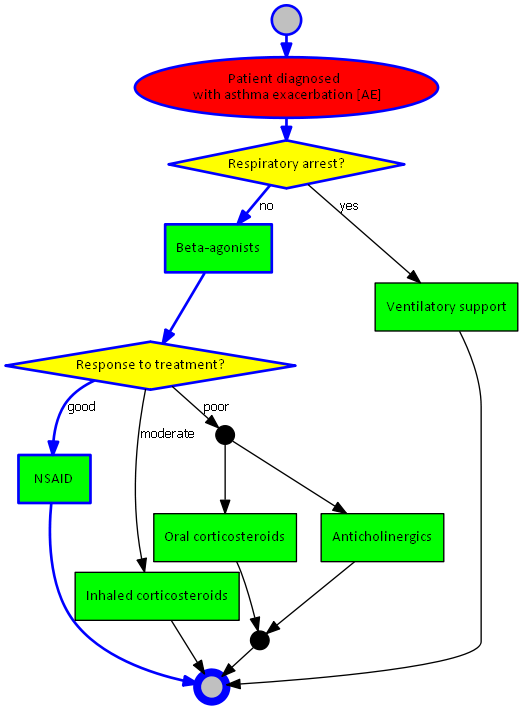
\includegraphics[width=0.7\textwidth]{img/asthma.png}
\end{figure}
\newpage
Wrzód trawienny (peptic ulcer) – graf:
\begin{figure}[H]
\centering
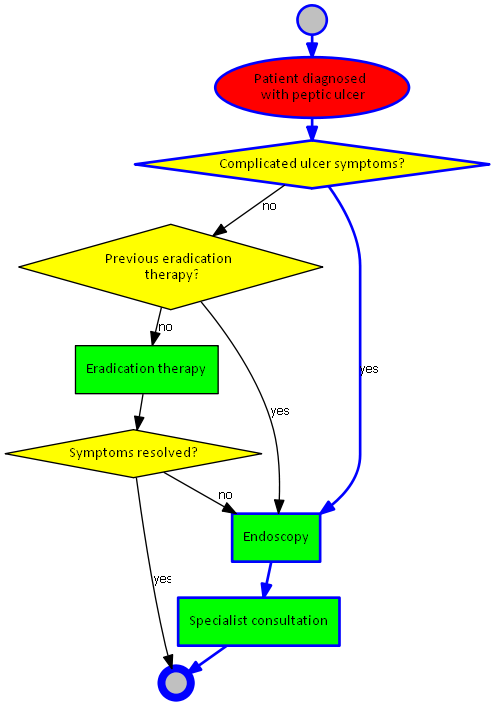
\includegraphics[width=0.7\textwidth]{img/peptic-ulcer.png}
\end{figure}
\newpage
\noindent Odpowiedzi na pytania:
\begin{enumerate}
\item{Atak astmy:
	\begin{itemize}
	\item{Respiratory arrest?: no}
	\item{Response to treatment?: good}
	\end{itemize}
}
\item{Wrzód trawienny:
	\begin{itemize}
	\item{Complicated ulcer symptoms?: yes}
	\end{itemize}
}
\end{enumerate}
Konflikty:
\begin{verbatim}
If diagnosed(PE) and execute(oral corticosteroids), then 
replace execute(oral corticosteroids) -> execute(inhaled corticosteroids)

If diagnosed(PE) and execute(NSAID)
then add execute(PPI) after execute(NSAID)

If execute(eradication therapy) and execute(inhaled corticosteroids), then
replace execute(inhaled corticosteroids) -> execute(oral corticosteroids)
\end{verbatim}
Znalezione konflikty:
\begin{verbatim}
If diagnosed(PE) and execute(NSAID) 
then add execute(PPI) after execute(NSAID)
\end{verbatim}
\newpage
\section{Przypadek 2 - migotanie przedsionków, przewlekła choroba nerek i nadciśnienie}

Migotanie przedsionków  (atrial fibrillation) – graf:
\begin{figure}[H]
\centering
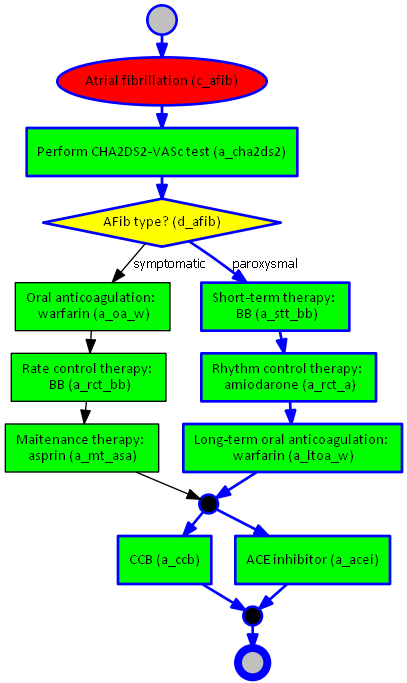
\includegraphics[width=0.7\textwidth]{img/afib-ver-4.png}
\end{figure}
\newpage
Przewlekła choroba nerek (chronic kidney disease) – graf:
\begin{figure}[H]
\centering
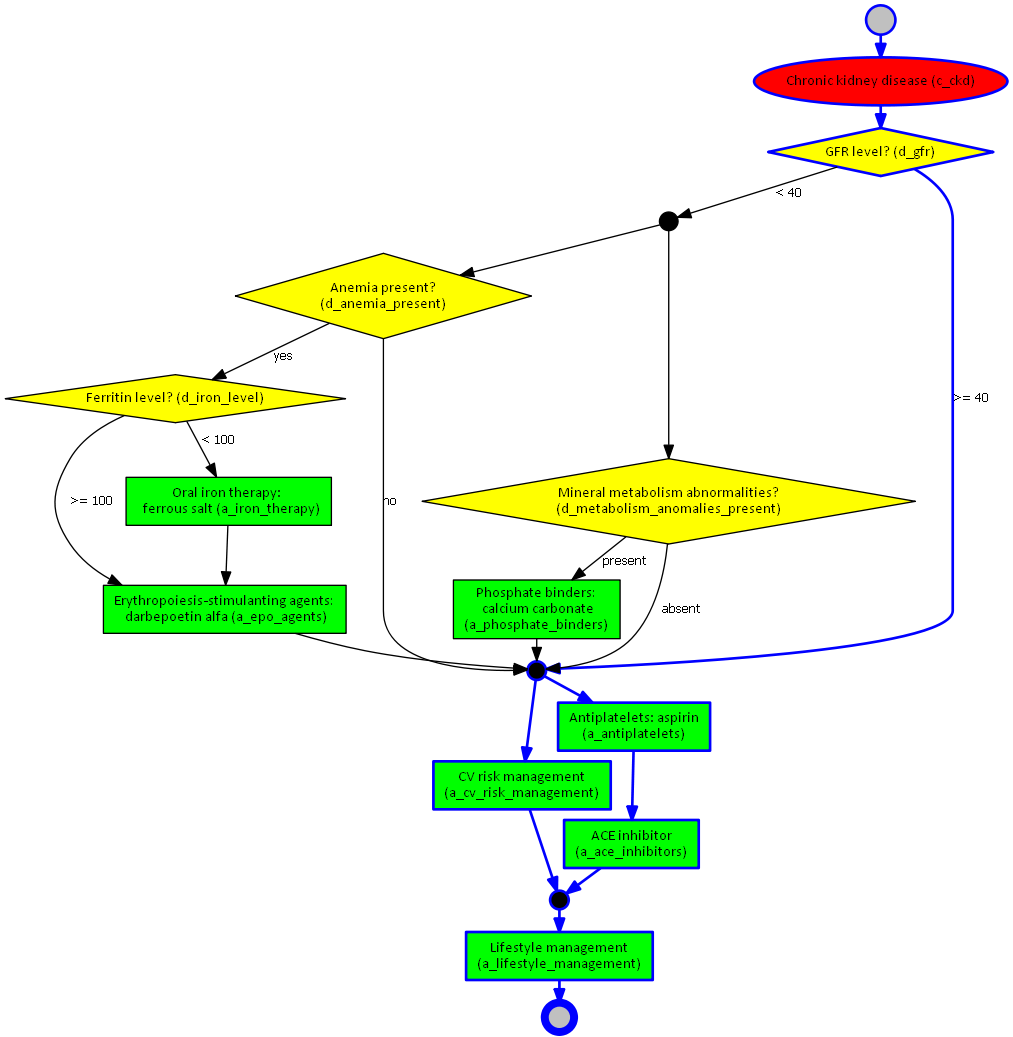
\includegraphics[width=0.8\textwidth]{img/ckd-simplified-ver-5.png}
\end{figure}
\newpage
Nadciśnienie (hypertension) – graf:
\begin{figure}[H]
\centering
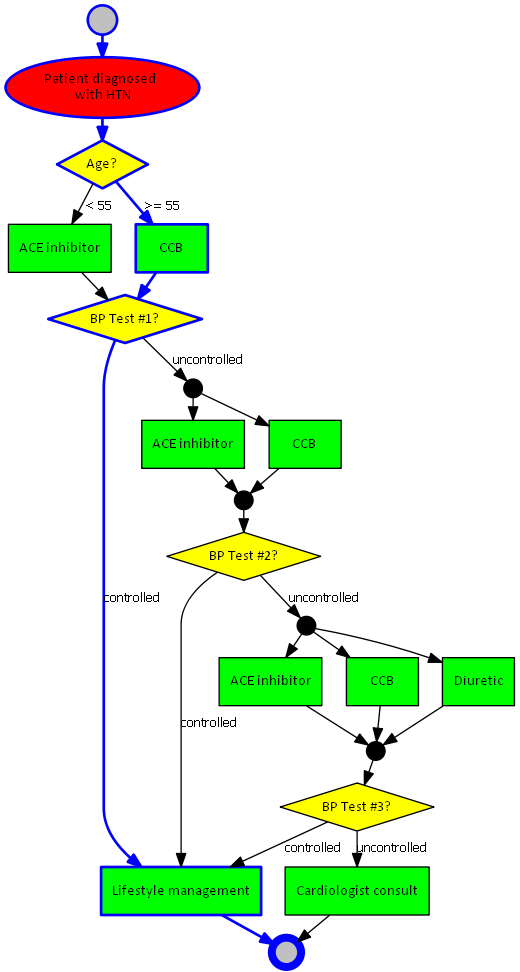
\includegraphics[width=0.7\textwidth]{img/htn-ver-3.png}
\end{figure}
\newpage
\noindent Odpowiedzi na pytania:
\begin{enumerate}
\item{Migotanie przedsionków:
	\begin{itemize}
	\item{AFib type?: paroxysmal}
	\end{itemize}
}
\item{Przewlekła choroba nerek:
	\begin{itemize}
	\item{GFR level?: >=40}
	\end{itemize}
}
\item{Nadciśnienie:
	\begin{itemize}
	\item{Age?: >=55}
	\item{BP Test \#1?: controlled}
	\end{itemize}
}
\item{CHA2DS2-VASc = 5}
\end{enumerate}
Konflikty:
\begin{verbatim}
If patient diagnosed with HTN and CKD, then remove Step 1 from the algorithm for HTN

If patient diagnosed with HTN, AFib and CKD, then delete “diuretics” from Step 3 
in the algorithm for HTN

If patient diagnosed with CKD and AFib, then replace aspirin with warfarin 
in the algorithm for CKD

If patient diagnosed with AFib and CKD, then replace amiodarone with BB 
in the algorithm for AFib

If patient diagnosed with AFib and CKD, and CHA2DS2-VASc > 2
then replace aspirin with warfarin as maintenance therapy in the algorithm for AFib

If patient diagnosed with Afib and CKD, and CHA2DS2-VASc <= 1
then replace warfarin with aspirin as the long-term therapy in the algorithm for AFib
\end{verbatim}
Znalezione konflikty:
\begin{verbatim}
If patient diagnosed with HTN and CKD, then remove Step 1 from the algorithm for HTN

If patient diagnosed with HTN, AFib and CKD, then delete “diuretics” from Step 3
in the algorithm for HTN

If patient diagnosed with CKD and AFib, then replace aspirin with warfarin 
in the algorithm for CKD

If patient diagnosed with AFib and CKD, then replace amiodarone with BB 
in the algorithm for AFib

If patient diagnosed with AFib and CKD, and CHA2DS2-VASc > 2
then replace aspirin with warfarin as maintenance therapy in the algorithm for AFib
\end{verbatim}
\newpage
\section{Przypadek 3 - wrzód dwunastnicy i przemijający atak niedokrwienny}

Wrzód dwunastnicy (duodenal ulcer) – graf:
\begin{figure}[H]
\centering
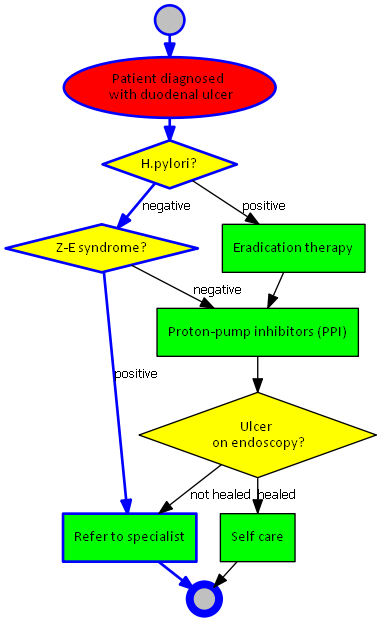
\includegraphics[width=0.7\textwidth]{img/du.png}
\end{figure}
\newpage
Przemijający atak niedokrwienny (transient ischemic attack) – graf:
\begin{figure}[H]
\centering
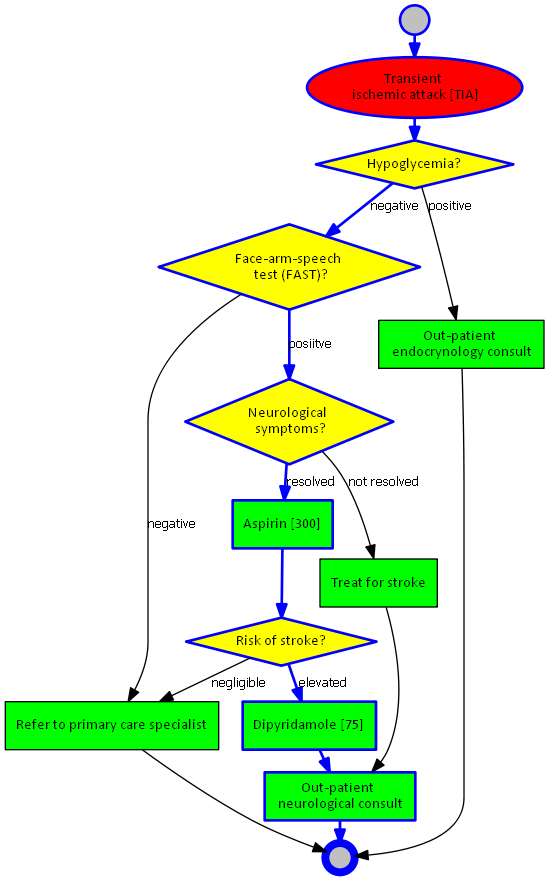
\includegraphics[width=0.7\textwidth]{img/tia.png}
\end{figure}
\newpage
\noindent Odpowiedzi na pytania:
\begin{enumerate}
\item{Wrzód dwunastnicy:
	\begin{itemize}
	\item{H.pylori?: negative}
	\item{Z-E syndrome?: positive}
	\end{itemize}
}
\item{Przemijający atak niedokrwienny:
	\begin{itemize}
	\item{Hypoglycemia?: negative}
	\item{Face-arm-speech test (FAST)?: positive}
	\item{Neurological symptoms?: resolved}
	\item{Risk of stroke?: elevated}
	\end{itemize}
}
\end{enumerate}
Konflikty:
\begin{verbatim}
if diagnosed(DU) and execute(A) and not execute(PPI) and not execute(D), then 
(1) replace execute(A) -> execute(CL)

if diagnosed(DU) and execute(A) and not execute(PPI) and execute(D), then
(1) replace not execute(PPI) -> execute(PPI) (wprowadź PPI)
(2) replace dosage(A, x) -> dosage(A, x – 50) (obniż dawkę A o 50 jednostek)
\end{verbatim}
Znalezione konflikty:
\begin{verbatim}
if diagnosed(DU) and execute(A) and not execute(PPI) and execute(D), then
(1) replace not execute(PPI) -> execute(PPI) (wprowadź PPI)
(2) replace dosage(A, x) -> dosage(A, x – 50) (obniż dawkę A o 50 jednostek)
\end{verbatim}

\chapter{Podsumowanie}

\section{Problemy przy realizacji projektu}

Do problemów przy realizacji pracy należy zaliczyć kwestię związaną z wyborem biblioteki służącej do przetwarzania grafów. Ostatecznie wybrana została biblioteka JPGD, ponieważ jest to dość prosta biblioteka. W bardzo łatwy sposób uzyskuje się dostęp do obiektu klasy Graph i podrzędnych obiektów klas Node oraz Edge. Niestety, skorzystanie z tej biblioteki wiązało się z naprawą pewnych błędów związanych z ponownym uzyskiwaniem grafu w wersji tekstowej. Konieczna była modyfikacja funkcji toString dla klas Graph, Node oraz Edge, ponieważ generowane początkowo przez bibliotekę grafy w wersji tekstowej nie pozwalały na wygenerowanie grafu w wersji obrazkowej przez program dot.exe. Przyczyna błędu tkwiła w tym, że biblioteka nie radziła sobie z pustymi wartościami atrybutów. Ponadto, trzeba było zrezygnować z korzystania z podgrafów, ponieważ były one niewłaściwie przez bibliotekę interpretowane.

\section{Kierunki dalszego rozwoju}

Podsumowując, wszystkie zamierzenia pracy zostały zrealizowane. Wynikiem pracy jest działający program wyszukujący konflikty występujące między stosowanymi terapiami chorób i proponujący rozwiązania ewentualnych konfliktów. Dalszy rozwój projektu mógłby dążyć do bardziej interaktywnej odpowiedzi na pytania. Program mógłby pozwalać na klikanie na krawędzie grafu zamiast wybierać odpowiedzi za pomocą radiobuttonów. Ponadto, program mógłby wspierać także inne formaty grafów, nie tylko format Graphviza o rozszerzeniu dot. 

\backmatter
\addcontentsline{toc}{chapter}{Bibliografia}
% rodzaj bibliografii
\bibliographystyle{plain}
% plik z wpisami bibliograficznymi
\bibliography{bibliografia}

\end{spacing}
\end{document}